% LAB 2: Basic Flow Control
% 
% CSE/IT 107: Introduction to Programming
% New Mexico Tech
% 
% Prepared by Russell White and Christopher Koch
% Fall 2014
\documentclass[11pt]{cselabheader}

%%%%%%%%%%%%%%%%%% SET TITLES %%%%%%%%%%%%%%%%%%%%%%%%%
\fancyhead[R]{Lab 2: Basic Flow Control}
\title{Lab 2: Basic Flow Control}

\begin{document}

\maketitle

\hrule

\begin{quotation}
``When you come to a fork in the road, take it."
\end{quotation}
\begin{flushright}
--- Attributed to Yogi Berra
\end{flushright}

\begin{quotation}
``Simplicity is the ultimate sophistication.''
\end{quotation}
\begin{flushright}
--- Leonardo Da Vinci
\end{flushright}

\begin{quotation}
``How do we convince people that in programming simplicity and clarity -- in
short: what mathematicians call elegance -- are not a dispensable luxury, but
a crucial matter that decides between success and failure?''
\end{quotation}
\begin{flushright}
--- Edsger Dijkstra
\end{flushright}

\hrule

\section{Introduction}
The purpose of this lab is to introduce you to the fundamentals of what
programmers call flow control. In the previous lab, we showed you how to do
basic calculations in Python. For example, we had you convert temperature from
Celsius to Fahrenheit and Kelvin.

What if the user of your conversion program wanted to have only one conversion
and you did not know which? We have to be able to give the user a choice. In the
previous lab, you learned about the \lstinline!input()! function that let you
``ask'' the user of your program a question. In this lab, you will learn how to
use \lstinline!if!, \lstinline!else!, and \lstinline!elif! to have the program
choose one action out of multiple actions; for example, whether to convert to
Kelvin or to Fahrenheit.

Sometimes, you also want to be able to repeat a calculation for different
values. For example, you want to calculate the square root of all numbers
between 1 and 100. To do this, you do not have to actually repeat writing the
calculation in your code, there is the \lstinline!while! statement to help you
repeat code.

\subsection{New Code Coloring in PDFs}

% also function names that are self-defined, but let's not talk about that..
In the new code style, all variable names will be black, all keywords will be
blue, all strings will be maroon (red), while comments are green. Any code that
is run in the Python interactive interpreter is on grey background.

%\begin{lstlisting}
%x = 5
%print(x)
%print("string")
%# I'm a comment
%\end{lstlisting}

\pagebreak
\section{Boolean Logic}

%Cover basic boolean logic with comparisons and whatnot, then use those to drive if and else statements.
A common activity when programming is determining if some value is true or
false. For example, checking if a variable is less than five or if the user
entered the correct password. Any statement that can be resolved into a true or
a false value is called a boolean statement, the value it resolves into (true or
false) is called a boolean value.

\begin{lstlisting}[style=ipython]
>>> x = 5
>>> print(x < 3)
False
>>> print(x < 6)
True
\end{lstlisting}

In the above example, the boolean values are \lstinline{True} and
\lstinline{False}. The boolean statements are \lstinline{x < 3} and 
\lstinline{x < 6}. 

In addition to \lstinline{<}, we can also test for other
inequalities.
\begin{lstlisting}[style=ipython]
>>> x = 3; y = 6
>>> print(x < y)
True
>>> print(x > y)
False
>>> print(x <= y)
True
>>> print(x >= y)
False
\end{lstlisting}

Note that \lstinline{<=} means ``less than or equal to'' and \lstinline{>=}
means ``greater than or equal to''. 

Finally, we can test if two values are equal
(\lstinline{==}) or not equal (\lstinline{!=}).
\begin{lstlisting}[style=ipython]
>>> x = 3; y = 3; z = 4
>>> print(x == y)
True
>>> print(x == z)
False
>>> print(y != 5)
True
>>> print(y != x)
False
\end{lstlisting}

It is important to remember that we use \lstinline{=} to assign a value to a variable and \lstinline{==} to test if two values are equal.

We can also combine boolean statements using \lstinline!and! and \lstinline!or!
as such:
\begin{lstlisting}[style=ipython]
>>> x = 3; y = 5; z = 8
>>> print(x < y and y < z)
True
>>> print(x > y and y < z)
False
>>> print(x > y or y < z)
True
>>> print(True and False)
False
>>> print(True or False)
True
\end{lstlisting}
If you combine two boolean statements that are true using \lstinline!and!, the
result will be true. In all other cases the result is false. Since 
\lstinline!x < y! is true and \lstinline!y < z! is true, we have that 
\lstinline!x < y and y < z! is true. See Table~\ref{tab:truth} for a ``truth
table'' showing what combinations are true or false -- it should make sense
though.

In addition to this, there is the \lstinline!not! operator to negate a boolean
statement. You can also put a boolean statement in parentheses to do more
complicated combinations:
\begin{lstlisting}[style=ipython]
>>> x = 3; y = 5; z = 8
>>> print(not True)
False
>>> print(not (x > y and y < z))
True
\end{lstlisting}

\begin{table}[!ht]
  \centering
  \begin{tabular}{ll | lll}
    \toprule
    \lstinline!A! & \lstinline!B! & \lstinline!A and B! & \lstinline!A or B! & \lstinline!not A! \\
    \midrule
    True & True & True & True & False\\
    True & False & False & True & False\\
    False & True & False & True & True\\
    False & False & False & False & True \\
    \bottomrule
  \end{tabular}
  \caption{Truth table}
  \label{tab:truth}
\end{table}

\subsection{Summary}

\begin{table}[!ht]
  \centering
  \begin{tabular}{ll}
    \toprule
    Comparison operator & What it tests\\
    \midrule
    \lstinline!a < b! & is $a$ less than $b$ \\
    \lstinline!a > b! & is $a$ greater than $b$ \\
    \lstinline!a <= b! & is $a$ less than or equal to $b$ \\
    \lstinline!a >= b! & is $a$ greater than or equal to $b$ \\
    \lstinline!a == b! & is $a$ equal to $b$ \\
    % because lstinline is retarded and doesn't work right in tables.
    \lstinline!a! !\lstinline!= b! & is $a$ not equal to $b$ \\
    \bottomrule
  \end{tabular}
  \caption{Comparison operators}
  \label{tab:cmpops}
\end{table}

\begin{table}
  \centering
  \begin{tabular}{ll}
    \toprule
    Boolean combination operator & What it does \\
    \midrule
    \lstinline!a and b! & true if both $a$ and $b$ are true \\
    \lstinline!a or b! & true if either $a$ or $b$ are true or both\\
    \lstinline!not a! & true if $a$ is false\\
    \bottomrule
  \end{tabular}
  \caption{Combination operators}
  \label{tab:cmbops}
\end{table}

\pagebreak
\section{Conditional Statements}

The primary use for boolean values is to determine which branch in your code to
follow. This is accomplished using \lstinline{if} and \lstinline{else}, as shown
in the program below. \lstinline!elif! will be introduced later in this lab. All
three -- \lstinline!if!, \lstinline!elif!, and \lstinline!else! -- are generally
called \emph{conditional statements}.

\begin{lstlisting}[style=python]
x = 1
y = float(input("Please input a number: "))

if x == y:
    print("x and y are equal.")
else:
    print("x and y are not equal.")
print("When do I print?")
\end{lstlisting}

Try running the above program, putting in different numbers for \lstinline{y}.
If the number input is 1, then the first \lstinline!print! statement will
output. If not, then the second one will. The third one will output regardless.

The way this works is very simple: either the first \lstinline!print! statement
runs or the second \lstinline!print! statement runs, but never both. Which one
runs is determined by Python: if the boolean statement (called \emph{condition})
following the \lstinline!if! evaluates to \lstinline!True!, then Python will
run the indented code following the \lstinline!if! and then skip until after
the indented code of the \lstinline!else!.

However, if the \emph{condition} evaluates to \lstinline!False!, then the
indented code following the \lstinline!else! is run and Python skips the
indented code between \lstinline!if! and \lstinline!else!.

It is important to note that the code that follows \lstinline!if! or
\lstinline!else! \textbf{must} be indented.

See what happens when you run the code below compared to the other piece of code
above:
\begin{lstlisting}
x = 1
y = float(input("Please input a number: "))

if x == y:
    print("x and y are equal.")
else:
    print("x and y are not equal.")
    print("When do I print?")
\end{lstlisting}

There are many uses for conditional statements, such as to ensure that a given
variable is not negative:

\begin{lstlisting}[style=python]
x = float(input("Please input a number: "))

if x < 0:
    x = 0 # sets x equal to 0 if x was less than 0

print("x = " + str(x))
\end{lstlisting}

You can perform other operations as part of a boolean statement, such as this convenient way to check if a number is even:

\begin{lstlisting}[style=python]
x = 5

if x % 2 == 0:
    print("x is even.")
else:
    print("x is odd.")
\end{lstlisting}

Remember that \lstinline!%! 
is the modulus operator: it gives you the remainder of the division.

When using \lstinline{if} and \lstinline{else}, you will generally be dealing
with user input. This is done using the function \lstinline{input}, which you
can see used in the above examples. When you use \lstinline{input} it will
display whatever string you pass to it, then pause while it waits for the user
to type something and then hit enter. It will give whatever was entered as a
string back to the variable that it is assigned to. We will be learning more
about strings in future labs, but for now just know that strings are basically
groups of letters, like what you pass to a \lstinline{print} statement, and are
declared by surrounding something in quotes.

The main thing to know about strings for now is that they cannot be used as
numbers. This is why we use the \lstinline{float} function to convert the string
the user gives us into a number.

\begin{lstlisting}[style=ipython]
>>> 5.5 == "5.5"
False
>>> 5.5 == float("5.5")
True
\end{lstlisting}

% PROBLEMS HERE HERE HERE
% ``float cannot run'' -- they dont know what that means.
It is important to understand the order that things happen in a statement like

\lstinline{x = float(input("Please input a number: "))}

Though both \lstinline{x = } and \lstinline{float} appear first in the line, the
first statement to execute is \lstinline{input}. This is because
\lstinline{input} is inside of \lstinline{float}'s parentheses and is therefore
being passed as a parameter to \lstinline{float}. Therefore, \lstinline{float}
cannot run until \lstinline{input} is finished and has returned a value to be
used by \lstinline{float}. Similarly, \lstinline{x = } will not happen until
\lstinline{float} has finished converting the value into a number.

If you are comparing strings, then you do not need to go through the extra step
of converting the user's input into a number:

\begin{lstlisting}[style=python]
password = "hunter2"

user_pass = input("Please input the password: ")

if password == user_pass:
    print("Password is correct. Welcome!")
else:
    print("Invalid password.")
\end{lstlisting}

In some cases, it could be that there are multiple passwords. Try running the
following code:
\begin{lstlisting}
password = "hunter2"
also_password = "hunter3"
another_password = "hunter4"
user_pass = input("Please input the password: ")

if password == user_pass:
    print("Welcome, administrator.")
elif user_pass == also_password:
    print("Welcome, administrator.")
elif user_pass == another_password:
    print("Welcome, manager.")
else:
    print("Wrong password.")
\end{lstlisting}

This introduced you to the \lstinline!elif! statement: When the condition
following \lstinline!if! turns out to be false, Python will then check the first
\lstinline!elif! statement. If that condition turns out to be true, it will run
the code following that \lstinline!elif! statement or move on to the next
\lstinline!elif!. Only if none of the conditions turned out to be true, the code
following \lstinline!else! will be run.

If you remember the boolean logic section, this problem could have been solved
more efficiently: two passwords are resulting in the same code. You could
rewrite the code like this:
\begin{lstlisting}
user_pass = input("Please input the password: ")

if user_pass == "hunter2" or user_pass == "hunter3":
    print("Welcome, administrator.")
elif user_pass == "hunter4":
    print("Welcome, manager.")
else:
    print("Wrong password.")
\end{lstlisting}

You can also nest the statements you just learned about. Try running the
following code, trying multiple values:
\begin{lstlisting}
x = float(input("Enter a value for x: "))
y = float(input("Enter a value for y: "))

if x > 0:
    if y > 0:
        print("Both are greater than 0.")
    else:
        print("x is greater than 0, but y is smaller or equal to 0")
else:
    print("x is smaller or equal to 0.")
\end{lstlisting}

\subsection{Summary}

\begin{itemize}
  \item Conditional statements look like this:
    \begin{lstlisting}
if condition:
    # some code to run
elif othercondition:
    # some other code to run
else:
    # alternative code if no condition was met
    \end{lstlisting}

  \item The \lstinline!elif! and \lstinline!else! sections are both optional
  \item \lstinline!elif! statements can be repeated as many times as you want.
  \item The conditions must be boolean statements.
  \item The code inside \lstinline!if!, \lstinline!elif!, and \lstinline!else!
    statements must be indented. Python will either show an error or behave very
    weirdly if you do not indent the code.
  \item You can nest conditional statements.
\end{itemize}

\subsection{Exercises}
\label{subsec:ifex}

\begin{description}
  \item[conversions.py] Use your \texttt{conversions.py} from last time and add a
    prompt asking the user whether to convert to Kelvin or Fahrenheit. It should
    look like this when it is run:

    \begin{lstlisting}[style=bash]
Please input the temperature in Celsius: 10
Please choose Kelvin (K) or Fahrenheit (F): F
You chose Fahrenheit.
Fahrenheit temperature: 50.0
    \end{lstlisting}
    \begin{lstlisting}[style=bash]
Please input the temperature in Celsius: 10
Please choose Kelvin (K) or Fahrenheit (F): K
You chose Kelvin.
Kelvin temperature: 283.15
    \end{lstlisting}
    \begin{lstlisting}[style=bash]
Please input the temperature in Celsius: 10
Please choose Kelvin (K) or Fahrenheit (F): E
You entered a letter I do not recognize.
    \end{lstlisting}

  \item[calculator.py] Write a small calculator that can compute arcsin, arccos,
    arctan and square root of a number. Use \lstinline!math.sqrt()!,
    \lstinline!math.asin()!, \lstinline!math.acos()!, and
    \lstinline!math.atan()!. Remember to import \lstinline!math!.

    \emph{Make sure to check for each function that the input is valid.} For
    example, for square root the input cannot be negative. For arcsin, the input
    must be between -1 and 1 inclusive. Try to figure out what the input must be
    for arccos and arctan yourself!

    \begin{lstlisting}[style=bash]
Enter a number to use: 16
Which operation? sqrt (s), arcsin (a), arccos (c), arctan (t): s
The square root of 16 is 4.0.
    \end{lstlisting}

    \begin{lstlisting}[style=bash]
Enter a number to use: 16
Which operation? sqrt (s), arcsin (a), arccos (c), arctan (t): a
16 is not in the domain of arcsin!
    \end{lstlisting}


\end{description}

\pagebreak
\section{Formatting Strings}

Previously, when we wanted to print out both a number and a string, we
had to resort to this:
\begin{lstlisting}[style=ipython]
>>> x = 5
>>> print("x is equal to " + str(x))
x is equal to 5
\end{lstlisting}

However, there is an easier way to accomplish the same thing. By using the
\lstinline!.format()! command, as shown below, we can have far more options for
how we format our output.

\begin{lstlisting}[style=ipython]
>>> x = 5
>>> print("x is equal to {}".format(x))
x is equal to 5
\end{lstlisting}

Rather than leaving a gap in our string and then using \lstinline{+} to add on
our variable, we instead include \lstinline!{}! where we wish to place our
variable and add on \lstinline{.format(x)} to the end of the string. This
replaces \lstinline!{}! with the value of \lstinline{x}.

If we include multiple instances of \lstinline!{}! in our string, we can then
pass multiple variables to \lstinline{.format()}. It will place them in the
string in the order provided.

\begin{lstlisting}[style=ipython]
>>> x = 5
>>> y = 6
>>> print("x is equal to {} and y is equal to {}.".format(x, y))
x is equal to 5 and y is equal to 6.
\end{lstlisting}

We can also use \lstinline!.format()! to control our output. For example, we can
restrict how many decimal places a floating point number is printed with. To do
this, we add \lstinline{:.2f} inside of the \lstinline!{}!. The \lstinline{.2f}
specifies that we want 2 digits to follow the decimal point. 
%If we wanted to, we
%could add an extra number before the colon to specify which of the arguments we
%want in this position. We don't want to mess with the order of the arguments, so
%we leave the position before the colon blank.

\begin{lstlisting}[style=ipython]
>>> import math
>>> print(math.pi)
3.141592653589793
>>> print("{:.2f}".format(math.pi))
3.14
\end{lstlisting}

For more format options, see
\begin{center}
  \vspace{-2mm}
\url{https://docs.python.org/3.1/library/string.html#format-string-syntax}
\vspace{-2mm}

\end{center}

\subsection{Summary}

\begin{itemize}
  \item Syntax:
    \begin{lstlisting}
print("string containing {}".format(variable))
    \end{lstlisting}
    
    This will replace the \lstinline!{}! with the value of \lstinline{variable}.
    
  \item You can include multiple \lstinline!{}! in a string and pass multiple values to \lstinline{format}.

  \item You can specify advanced formatting options, such as number of digits after the decimal point.
\end{itemize}

\pagebreak
\section{Loops}
%Apply the above to while loops.

\subsection{While Loops}
The syntax of a \lstinline{while} loop is very similar to that of an
\lstinline{if} statement, but instead of only running the indented block of code
once, the \lstinline{while} loop will continue running it until the given
boolean statement is no longer true.

\begin{lstlisting}[style=python]
x = 10

while x > 0:
    print(x)
    x = x - 1
\end{lstlisting}

The above program will print out the numbers 10 to 1. Try stepping through this
program on paper, writing out the value of \lstinline{x} at each time through
the loop. Then repeat for this modified version of the program:

\begin{lstlisting}[style=python]
x = 10

while x > 0:
    x = x - 1
    print(x)
\end{lstlisting}

This version of the program will print out the numbers 9 to 0. This might seem a
bit strange, since the condition of the loop says it will stop when
\lstinline{x} is no longer larger than 0. And yet, it prints out the value 0
before the loop ends. This is because the loop condition is only checked
whenever the end of the indented section is reached. If the condition is
\lstinline{True}, then the indented section will be executed again. If the
condition is \lstinline{False}, then the loop will end.

If the condition starts out \lstinline{False}, then the loop will never execute.
The following program will not print anything:

\begin{lstlisting}[style=python]
x = 0

while x > 0:
    x = x - 1
    print(x)
\end{lstlisting}

\lstinline{if} and \lstinline{else} can be combined with \lstinline{while}, as
shown below:

\begin{lstlisting}[style=python]
x = 10

while x > 0:
    if x % 2 == 0:
        print("{} is even.".format(x))
    else:
        print("{} is odd.".format(x))
    x = x - 1
\end{lstlisting}

Of course, they can be nested the other way around, too, with a
\lstinline!while! inside conditional statements.

There can also be infinite while loops. Try the following:
\begin{lstlisting}
while True:
    print("Printing forever")
\end{lstlisting}

Press \emph{Ctrl+C} to stop the execution of this.

\subsection{For Loops}

Instead of using \lstinline!while! loops, you can also use the \lstinline!for!
iterator (often also called \lstinline!for! loop). The \lstinline!for! loop
allows you to ``iterate'' over a given list of things, for example a list of
characters (a string):
\begin{lstlisting}
for c in "abc":
    print("Hi, {}!".format(c))
\end{lstlisting}

Here, \lstinline!c! is a variable you can use inside the code block of the
for loop.

The example will print:
\begin{lstlisting}[style=bash]
Hi, a!
Hi, b!
Hi, c!
\end{lstlisting}

A for loop can be over numbers as well, but this requires us to use the
\lstinline!range()! function. You can give \lstinline!range()! a starting number
and an end number:
\begin{lstlisting}
for num in range(0, 10):
    print(num)
\end{lstlisting}
This will print the numbers from \emph{zero} to \emph{nine}. Notice that 10 is
not included!

You can also give \lstinline!range()! a starting number, an end number, and an
increment. The increment can be positive or negative. The numbers do not have to
be actual numbers, you can give variables to it, too:
\begin{lstlisting}
start = 10
end = 0
increment = -2
for number in range(start, end, increment):
    print(number)
\end{lstlisting}
This will print:
\begin{lstlisting}[style=bash]
10
8
6
4
2
\end{lstlisting}
Notice how zero is not included. The end number is never included when you use
\lstinline!range()!.

You can also just have the \lstinline!for! loop ``iterate'' over a list of
things:
\begin{lstlisting}
for number in [0, -2, 20, 24]:
    print(number)
\end{lstlisting}

\pagebreak
\subsection{Nesting}

You can nest for loops and while loops and conditional statements in any way you
like. The following is just an example:
\begin{lstlisting}
parity = input("Even or odd? ")

# prints even or odd numbers between 0 and 10, depending on user input
if parity == "odd":
    for n in range(1, 11, 2):
        print(n)
elif parity == "even":
    n = 0
    while n <= 10:
        print(n)
        n = n + 2
else:
    print("You did not enter even or odd.")
\end{lstlisting}

\subsection{Summary}

\begin{itemize}
    \item Syntax:
      \begin{lstlisting}
while condition:
    # code to be repeated
      \end{lstlisting}

    This will repeat the indented code following the \lstinline!while! until the
    condition is not true anymore. It checks the condition first, then runs the
    indented code, then checks the condition again, etc. Thus, if the condition
    is wrong in the first place, it will never run.

  \item Syntax:
    \begin{lstlisting}
for variable in list:
    # code doing something with variable
    \end{lstlisting}

    The list can be a string or a \lstinline!range()! function or an actual list
    delimited by brackets \lstinline![]!. You will soon
    learn that there is also a list data type in Python that you can use here
    and other nice things, but we do not cover that in this lab.

  \item There can be infinite while loops.
  \item You can nest conditional statements and loops any way you want in any
    combination.
\end{itemize}

\pagebreak
\subsection{Exercises}
\label{subsec:whileex}

\begin{description}
  \item[fizzbuzz.py] Have the user enter a positive integer number. Then, print
    the numbers from 1 to that number each on a line. When the printed number is
    divisible by 3, print ``Fizz'', and when the number is divisible by 5, print
    ``Buzz'', and when it is divisible by both, print ``FizzBuzz''.

    You must use \lstinline!.format()! and a \lstinline!while! loop.

    Should look like this when run:
    \begin{lstlisting}[style=bash]
Enter a number: 16
1
2
3 Fizz
4
5 Buzz
6 Fizz
7
8
9 Fizz
10 Buzz
11
12 Fizz
13
14
15 FizzBuzz
16
    \end{lstlisting}
    \begin{lstlisting}[style=bash]
Enter a number: -1
Not a positive number!
    \end{lstlisting}

  \item[fizzbuzz\_for.py] Write the same fizzbuzz program using a
    \lstinline!for! loop and \lstinline!range()! this time. Using
    \lstinline!.format()! is still required.

  \item[primes.py] (Practice of Computing Using Python \#2.15) Write a program that checks if a number
    $N$ is prime. You have to ask the user for the number. Remember that a prime
    number is a number that is divisible only by $1$ and itself.

    A simple approach checks all numbers from $2$ up to $N$.

    Try to improve on the simple approach, though: do we really need to check
    all those numbers? At which point do you know that you can stop? Remember to
    import \lstinline!math!.

  \item[dna.py] 
    DNA is generally encoded with four letters: A, T, G, and C. For example, a
    string of DNA would be ``ATTGCAT''.

    You can find the ``complement'' of DNA for some biological reason (it is
    double stranded, but that does not matter to us). The complement of A is T
    and vice versa; the complement of G is C and vice versa.

    Write a program that takes in a strand of DNA from the user using
    \lstinline!input! and finds its complement. Assume the user always enters
    valid DNA made up of the four letters.

    \begin{lstlisting}[style=bash]
Enter DNA: ATTGCAT
Complement is: TAACGTA
    \end{lstlisting}

\end{description}

\pagebreak
\section{Turtle}

%Cover how to use turtle, give an example of a program to use a while loop to draw a hexagon or something.
Some of the exercises for this lab will use Turtle, a simple graphics library.
It can be accessed by using \lstinline{import turtle} in Python. From there you
have access to a group of functions for controlling the ``turtle'', a simple
arrow that moves around at your command, drawing a line where it goes. The
primary commands to control the turtle are shown in Table \ref{tab:turtle}.

\begin{table}[h]
  \centering
  \begin{tabular}{ll}
    \toprule
    Operator & What it does\\
    \midrule
    \lstinline!turtle.forward(x)! & move the turtle forward \lstinline!x! pixels \\
    \lstinline!turtle.backward(x)! & move the turtle backward \lstinline!x! pixels \\
    \lstinline!turtle.left(x)! & turn the turtle left \lstinline!x! degrees \\
    \lstinline!turtle.right(x)! & turn the turtle right \lstinline!x! degrees \\
    \bottomrule
  \end{tabular}
  \caption{Turtle commands}
  \label{tab:turtle}
\end{table}

It should be noted that giving a negative value to these commands is allowed, so
\lstinline!turtle.left(-30)! is equivalent to \lstinline!turtle.right(30)!.

Combining these commands will let you draw potentially complex shapes. For
example, the following program will draw a hexagon.

\begin{lstlisting}[style=python]
import turtle

turtle.forward(100)
turtle.left(60)
turtle.forward(100)
turtle.left(60)
turtle.forward(100)
turtle.left(60)
turtle.forward(100)
turtle.left(60)
turtle.forward(100)
turtle.left(60)
turtle.forward(100)
turtle.left(60)
\end{lstlisting}

However, this code is a bit longer than it needs to be. Let's clean it up a bit using \lstinline{while}.

\begin{lstlisting}[style=python]
import turtle

counter = 0

while counter < 6:
    turtle.forward(100)
    turtle.left(angle)
    counter = counter + 1
\end{lstlisting}

\pagebreak
\subsection{Exercises}
\label{subsec:turtleex}

\begin{description}

  \item[star.py] Write a program that draws a shape like the picture below.

    \begin{figure}[!ht]
      \centering
      
\includegraphics[width=1.0in]{img/star}
      % Picture and exercise taken from
      % http://openbookproject.net/thinkcs/python/english3e/hello_little_turtles.html
      % public under GNU license
      % Copyright of Peter Wentworth, Jeffrey Elkner, Allen B. Downey and Chris Meyers
    \end{figure}

    Hint: Try this on paper first. (It does not matter if the turtle is still
    displayed when it is drawn.)

  \item[polygons.py] Write a program that takes in a number using
    \lstinline{input} and then draws a regular polygon with that many sides. A
    regular polygon is one where each side is the same length and each corner is
    the same angle. For example, the sample code given in the section draws a
    regular hexagon.

    Input:
    \begin{lstlisting}[style=ipython]
How many sides? 3
    \end{lstlisting}

    Output:
    \begin{figure}[h]
      \centering
%      \vspace{-10mm}
      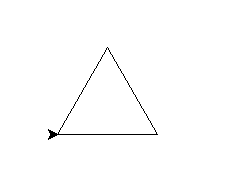
\includegraphics[width=2.0in]{img/triangle}
%    \vspace{-10mm}
    \end{figure}

  \item[navigate.py] Write a program that takes directions from the command line
    to draw a line. Let the user input ``left'', ``right'', ``forward'', or
    ``stop''. Left and right turn the turtle left or right however many degrees
    are entered, forward moves the turtle forward (however far you wish), and
    stop ends the program. Please check the degrees for errors: they must be
    between 0 and 360 degrees! (Yes, Turtle could handle negative degrees, but
    we would like you to check.)

    Input:
  \begin{lstlisting}[style=bash]
Please enter a direction: forward
Please enter a direction: left
How many degrees? 45
Please enter a direction: forward
Please enter a direction: left
How many degrees? -1
Invalid number, not moving.
Please enter a direction: left
How many degrees? 45
Please enter a direction: forward
Please enter a direction: forward
Please enter a direction: left
How many degrees? 45
Please enter a direction: left
How many degrees? 45
Please enter a direction: forward
Please enter a direction: right
How many degrees? 45
Please enter a direction: forward
Please enter a direction: stop
  \end{lstlisting}

    Output:
  \begin{figure}[!ht]
    \centering
%    \vspace{-5mm}
    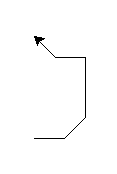
\includegraphics[width=1.0in]{img/navigate}
%    \vspace{-10mm}
  \end{figure}


\end{description}

\pagebreak

\section{Submitting}

Files to submit:
\begin{itemize}
  \item conversions.py (see Section~\ref{subsec:ifex})
  \item calculator.py (see Section~\ref{subsec:ifex})
  \item fizzbuzz.py (see Section~\ref{subsec:whileex})
  \item fizzbuzz\_for.py (see Section~\ref{subsec:whileex})
  \item primes.py (see Section~\ref{subsec:whileex})
  \item dna.py (see Section~\ref{subsec:whileex})
  \item polygons.py (see Section~\ref{subsec:turtleex})
  \item navigate.py (see Section~\ref{subsec:turtleex})
  \item star.py (see Section~\ref{subsec:turtleex})
\end{itemize}

You may submit your code as either a tarball (instructions below) or as a .zip
file. Either one should contain all files used in the exercises for this lab.
The submitted file should be named either
\texttt{cse107\_firstname\_lastname\_lab2.zip} or
\texttt{cse107\_firstname\_lastname\_lab2.tar.gz} depending on which method you
used.

For Windows, use a tool you like to create a \texttt{.zip} file. The TCC computers should
have \texttt{7z} installed. For Linux, look at lab 1 for instructions on how to
create a tarball or use the ``Archive Manager'' graphical tool.

\begin{center}
  \textbf{Upload your tarball or .zip file to Canvas.}
\end{center}

\end{document}
